\documentclass[10pt, a4paper]{article}
\usepackage[T2A]{fontenc}
\usepackage[english, russian]{babel}

\usepackage{graphicx}
\graphicspath{{./figs/}}

\usepackage{amsmath}
\usepackage{amssymb}
\usepackage{mathtools}
\usepackage{physics}
\usepackage{upgreek}
\usepackage{sectsty}
\usepackage{color,soul}
\usepackage[colorlinks=true,allcolors=blue]{hyperref}
\sectionfont{\centering}

\usepackage{geometry}
 \geometry{
 a4paper,
 margin=25mm,
 }

\title{Билеты к кандидатскому экзамену по физике плазмы}
\date{}

\begin{document}

\newpage
\section{Термодинамика плазмы}
\label{sec.1}

\subsection{Понятие плазмы, квазинейтральность, микрополя, дебаевский радиус, идеальная и неидеальная плазма.}
\label{sec.1.1}

Плазма~\cite{kotelnikov}. Ссылка на уравнение~\eqref{eq.Euler}, Рис.~\ref{fig.1.2.1}.

У плазмы вводят т.н. параметр неидеальности, который есть $g = \frac{1}{n * r_d^3}$(Kroll, eq. 1.3.1). Когда 
$g \ll 1$ говорят, что плазма идеальна, т.к. в этом случае её свойства, как газа, схожи с идеальным газом.



~\cite{kotelnikov}. Ссылка на уравнение~\eqref{eq.Euler}, Рис.~\ref{fig.1.2.1}.


\begin{equation}
    \label{eq.Euler}
    e^{i \pi} + 1 = 0
\end{equation}

\subsection{Условие термодинамического равновесия, термическая ионизация, формула Саха, корональное равновесие, снижение потенциала ионизации.}
\label{sec.1.2}

Картинка

\begin{figure}[h!]
    \center{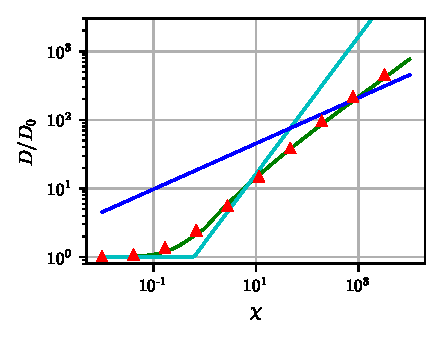
\includegraphics[width=85mm]{test.pdf}}
    \caption{\label{fig.1.2.1} Подпись.}
\end{figure}

\subsection{Вырождение плазмы, статистика Больцмана и Ферми—Дирака, модель Томаса—Ферми.}


\section{Элементарные процессы}
\label{sec.2}

\subsection{Столкновения заряженных частиц, дальнодействие.}
\label{sec.2.1}

[Ю.П. Райзер, Физика Газового разряда, 3-е изд, стр. 29]

Из всех сил взаимодействия между атомными частицами медленнее вceгo спадают с расстоянием (как $1/r^{2}$)  кулоновские силы. Они обладают наибольшим дальнодействием.
За время пролёта t мимо иона, электрон отклоняется на угол $\theta$ . Его можно оценить как отношение полученной поперечной скорости к изначальной скорости:

Основную роль в рассеянии играют столкновения с большим прицельным параметром $\rho$ (рассеяние на малые углы),реализуются при  $\rho > r_{0}$- Кулоновского радиуса (радиус при котором кин. энергия электрона равна потенциальной $ mv^{2}/2 = e^{2}/ r_{0} $,$ r_{0}=e^{2}/mv^{2} $). С другой стороны, потенциал иона спадает $\sim exp(-r/d)/r $. То есть основной вклад вносят столкновения с прицельным параметром от  $r_{0}$   до $d$ (радиус дебая).
Поэтому полное сечение для кулоновских рассеяний $\sigma= \pi*r_{0}^{2} \int_{r_{0}}^{d} r_{0} d\rho/\rho =\pi*r_{0}^{2}*ln{d/r_{0}}$

$ln{d/r_{0}}$ - Кулоновский логарифм.

Столкновения атомных частиц могут иметь упругий и неупругий характер. При упругом соударении меняются направления движения партнеров, происходит обмен импульсом и кинетической энергией, но внутренние энергии и состояния частиц остаются неизменными.

\subsection{Частоты столкновений}
\label{sec.2.2}

[Ю.П. Райзер, Физика Газового разряда, 3-е изд, стр.20]

Число соударений определенного рода, которые данная частица (назовем: ее 1) в среднем совершает в 1 с, двигаясь в газе из частиц мишеней 2, называют частотой столкновений.

$\nu_{1}=N_{2}*v'*\sigma (v')$
, где $v'$ скорость сближения

Для газовой кинетики это тоже работает и если распределение частиц массы М по абсолютным скоростям описывается максвелловской функцией, то вместо скорости надо ставить среднее её значение $\bar{v'}=\sqrt{2} \bar{v}$ ; $\bar{v}=\sqrt{\frac{8kT}{\pi M}}$, где за массу надо брать приведённое её значение по 2-м частицам ($ M=\frac{M_{1} M_{2}}{(M_{1}+M_{2})} $), а за сечение рассеяния $\pi d_{mol}^{2} $

\subsection{Столкновения электронов с атомами (упругие и неупругие)}
\label{sec.2.3}


\subsubsection{Упругие}
\label{sec.2.3.1}
[Астапенко В.А.,Лисица В.С., столкновительные процессы в …... стр.30]


Вычисление сечения процесса является сложным кванто-механическим расчетом и зависит от скорости налетающего электрона. Транспортное сечение выражается сложным образом
\begin{equation}
\sigma_{tr}=4\pi (L^{2}+\frac{4}{5}\frac{\pi \alpha L}{a_{bor}}\frac{mV}{\hbar}+\frac{\pi^{2}}{6}\frac{\alpha^{2}}{a_{bor}^{2}}(\frac{mV}{\hbar})^{2})
\end{equation}
Здесь $L$ - длина рассеяния электрона на атоме. Первый член - короткодействующие силы. Последний - дальнодействующий потенциал деполяризационный. Промежуточный - интерфериционный от предыдущих двух (проявляются волновые свойства электрона), он может быть отрицательным (при отрицательном L).
Как именно происходит интерференция - см [И. мак-Даниэль, процессы столкновений в ионизированных газах,гл. 4, §4, стр 161] и [гл. 3, §15, пункт Д, “рассеяние  S волны на сферической потенциальной яме”]

\subsubsection{Неупругие}
\label{sec.2.3.2}

Ионизация

[Астапенко В.А.,Лисица В.С., столкновительные процессы в …... стр.37]

Так как после ионизации мы имеем ситуацию, что электрон улетает от иона, то это мы можем рассматривать как упругое рассеяние электрона на ионе, однако в сечение войдут не все электроны, а лишь с энергией выше, чем $E_{ion}$

$\frac{d\sigma^{(R)}}{d\Omega}=(\frac{Ze^{2}}{2mV^{2}sin^{2}(\frac{\theta}{2})})^{2}$

При рассеянии иону передается импулmc $\Delta p=2mVsin(\theta/2)$ и соответственно энергия $\Delta E=4 E sin^{2}(\theta/2)$ , поэтому можно перейти к интегрированию по энергиям.
$\delta \sigma =\frac {\pi e^{2}d\Delta E}{E(\Delta E)^2}$; 
$\sigma_{ion}=\int_{E_{ion}}^{E} d\sigma=\frac{\pi e^4}{E}(\frac{1}{E_{ion}}-\frac{1}{E})=\frac{\pi e^4}{E_{ion}^{2}}\frac{x-1}{x}$
, где $x=E-E_{ion}$ , то есть ионизация имеет пороговый характер


Возбуждение электронным ударом [Астапенко В.А.,Лисица В.С., столкновительные процессы в …... стр.50]


Уравнение рассматриваемого процесса имеет вид $e + A -> A* + e$. Согласно этому принципу атом при взаимодействии с электромагнитным полем ведёт себя как набор осцилляторов, которые ставятся в соответствие паре энергетических уровней $E_i$ , $E_j$ атомного спектра. Собственные частоты этих осцилляторов равны собственной частоте перехода $i -> j$ , $\omega _{i,j}=\frac{(E_j-E_i)}{\hbar}$ , а эффективность их взаимодействия с электромагнитным полем определяется силой осциллятора:
\begin{equation}
f_{i,j}=\frac{2m\omega_{ij} {|d_{ij}|}^{2} }{3\hbar e^{2} g_i}
\end{equation}

, где $g_i$ - статистический вес начального состояния. 

При кванто-механическом описании дипольный момент осциллятора перехода $d_{ij}$ представляет собой матричный элемент ооператора электрического дипольного момента между состояниями $|i>$, $|j>$. В случае возбуждения атома $i,j>0$ и $f_{i,j}>0$, для электронного перехода с уменьшением энергии $i,j<0$ и $f_{i,j}<0$. Также может быть $f_{i,j}=0$, тогда такие переходы называются дипольно-(или оптически) запрещенными. Если  $f_{i,j} \ne 0$ оптически-разрешенный переход.
Предполагая поле налетающего электрона в области локализации атома однородным, можно записать следующее уравнение для радиус-вектора осциллятора $rij$:
$r_{ij}''+\gamma_{ij}r_{ij}'+\omega_{ij}^{2}r_{ij}=f_{i,j}\frac{e}{m}E(t,\rho)$, где $\gamma_{ij}$-константа затухания,  $\rho$- прицельный параметр. Записывается скорость затухания в таком осцилляторе и ищется работа, которую совершает поле над осциллятором за всё время столкновения.
Вероятность возбудить атом будет $W_{ij}(\rho)=\frac {A_{ij}(\rho)}{\hbar_{ij}}$, полное сечение  будет $\sigma_{ij}=2\pi \int_{a}^{\inf} W_{ij}(\rho)\rho d\rho$. Тут, как и в кулоновском рассеянии основную роль играют рассеяние на малые углы, то есть с большим прицельным параметром.
\begin{equation}
\sigma_{ij}=\pi f_{ij} \frac {e^{2}}{m\Delta E_{ij} } \int_{a}^{\inf} |E(\omega_{ij},\rho)|^{2} \rho d\rho
\end{equation}
Далее - трудные выкладки с методом функции подобия. Самое главное, характер функции сигмы от энергии. Она выглядит схожим образом с зависимостью сечения ионизации. Также имеет пороговый характер, на бесконечности спадает как $ln(E)/E$. Имеет максимум в при $E=3,45*E_{ij}$
Для запрещенных переходов данный расчёт в дипольном приближении невозможен. ибо носит не дипольный характер. Дипольно-запрещённые переходы бывают двух типов: без изменения спина атома (дипольный момент перехода отсутствует из-за невыполнения правил отбора по орбитальному квантовому числу L, переход осуществляется за счёт прямого кулоновского взаимодействия) и переходы с изменением атомного спина (В этом случае возбуждение атома происходит за счет обменного взаимодействия между налетающим и атомным электроном).



\subsection{столкновения тяжелых частиц}
\label{sec.2.4}


[Астапенко В.А.,Лисица В.С., столкновительные процессы в …... стр.90]

Столкновения заряженных тяжелых частиц (ионов) с атомами и молекулами зависит, как и столкновения тяжелых нейтральных частиц, от поведения термов сталкивающихся партнеров. Эволюция во времени термов квазимолекулы, образованной сталкивающимися атомами, схематически представлена на рис. 
Переходы могут быть быстрыми (барновские) и медленные (адиабатические). В частности если будем рассматривать термы квазимолекулы, образованной сталкивающимися атомами. Зависимость потенциала от времени обусловлена их зависимостью траектории от времени.
Понятно, что с какой-то вероятностью электрон может перескочить с одного уровня на другой.

\begin{figure}[h!]
	\center{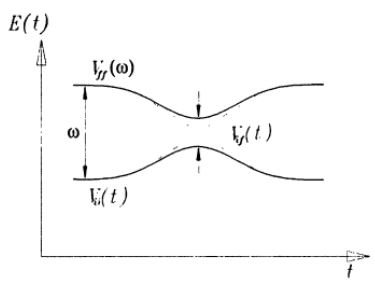
\includegraphics[width=70mm]{heavy_particle.JPG}}
	%\caption{\label{fig.2.4.1}}
\end{figure}



\subsection{Резонансная перезарядка}
\label{sec.2.5}

Резонансная перезарядка. Состоит в передаче электрона от одного ядра к другому в системе идентичных ядер: $A + A^{+} \rightarrow A^{+} + A$. Здесь, на первый взгляд, начальные и конечные состояния системы совпадают. Надо помнить, однако, что при этом происходит обмен скоростями между нейтральным атомом и ионом(направления движения каждого останется прежним)

Взаимодействие $V(R)$ в  определяющее переход электрона от одного ядра (атом) к другому (ион), определяется перекрытием волновых функций на двух ядрах, разделенных  
расстоянием $R$: $V(R)=exp(-\gamma R)$($\gamma=(2I)^{1/2}$ - определяется энергией связи $I$ электрона в атоме). Фактически при перезарядке электрон туннелирует между двумя потенциальными ямами.

\begin{figure}[h!]
	\center{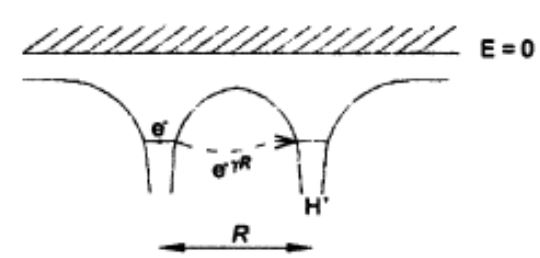
\includegraphics[width=70mm]{res_recharge.JPG}}
	%\caption{\label{fig.2.4.2}}
\end{figure}
 Вероятность перехода:
\begin{equation}
w(\rho)=sin^{2}[ \int_{-\inf}^{+inf} V(R(t))dt] \sim sin^{2}[V(\rho)\rho/v]
\end{equation}
Как следует из формулы, вероятность перехода между двумя ядрами быстро осциллирует при малых относительных скоростях v в соответствии с многократным перескоком электрона от одного ядра к другому, в результате чего электрон в среднем с вероятностью 1/2  находится в потенциальной яме каждого из ядер. Интегрируя свесом $2\pi\rho d\rho$, получим сечение резонансной перезарядки:
\begin{equation}
\sigma_{res}\propto(frac{pi}{2\gamma^{2}})ln^{2}(v_0/v)
\end{equation}

, где $v_0$ - скорость электрона на атомной орбите (порядка атомной). Видно, что сечение резонансной перезарядки значительно превышает атомные сечения благодаря большому значению логарифма  отношения атомной скорости к скорости относительного движения ядер.  Например, это сечение равно $5*10^{-15} см^{2}$ для перезарядки протона на водороде при энергии 1 эВ.

P.S. есть ещё и нерезонансная перезарядка при нерезонансной перезарядке, соответствующей передаче электрона от одного ядра к другому в случае неидентичных ядер с разными энергиями 
связи электрона на каждом из них.

Особый случай соответствует перезарядке атома на многозарядном ионе, потенциал ионизации которого намного превосходит потенциал ионизации исходного атома. Здесь атомный электрон переходит в густой спектр высоковозбужденных состояний многозарядного иона, для которых энергия связи близка к энергии связи в исходном атоме.
\begin{figure}[h!]
	\center{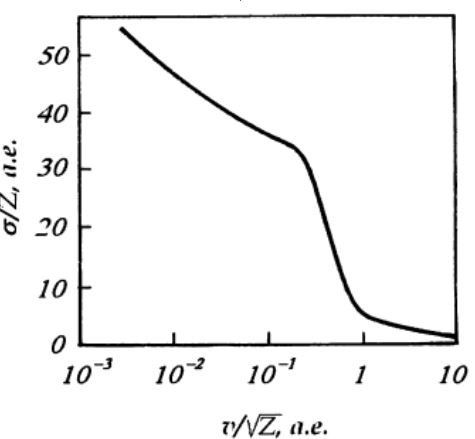
\includegraphics[width=70mm]{res_recharge_1.JPG}}
	%\caption{\label{fig.2.4.2}}
\end{figure}

Наверное, из всего надо вынести то, что при малых скоростях/энергиях налетающего атома, сечение будет большим, чтобы электрон за большое время пролёта стуннелировал в другой атом/ион. Экспериментально это и было подтверждено.(см рис.) В случае сильно искривлённого поля иона, туда ему стунелировать гораздо проще, поэтому сечение перезарядки $\sim Zn^{4}$, где z - заряд иона, n- номер орбиты

\subsection{Рекомбинация}
\label{sec.2.6}
Рекомбинация [Астапенко В.А.,Лисица В.С., столкновительные процессы в …... стр.99]


Трехчастичная рекомбинация является процессом, детально обратным процессу ионизации и, следовательно, записывается уравнением $A^{+Z} + 2e -> A^{+(Z-1)} + e $.Суть процесса трехчастичной рекомбинации состоит в том, что электрон плазмы, взаимодействующий с ионом, отдает избыток своей энергии другому электрону плазмы и захватывается на  уровень иона. Ясно, что рассматриваемый процесс может играть доминирующую роль в плазме с достаточно высокой плотностью (чтобы присутствие третьей частицы было вероятным) и низкой температурой (чтобы радиус кулоновского взаимодействия между частицами был велик). Оценим скорость рекомбинации:
\begin{equation}
\alpha_3 n^2_e N_i = k_{step} N_{neutr} n_e
\end{equation}

Подставляя из Саха-больцмана значение для соотношения $\frac{N_e N_i}{N_{neut}}$ получаем оценку для скорости ступенчатой ионизации
\begin{equation}
	k_{step}=\frac{C}{(2\pi)^{3/2}}\frac{g_i}{g_a}\frac{me^{10}}{\hbar^{3}T^{3}}exp(-I/T)
\end{equation}

Для сравнения этой скорости со скоростью прямой ионизации ($k_{dir}$)(как бы ионизация напрямую электроном с энергией равной энергии ионизации):
 \begin{equation}
 	k_{dir}=v_{el} \sigma_{dir}=\sqrt{2T/m} a_{0}^{2} exp(-I/T)
 \end{equation}

 \begin{equation}
 		\frac{k_{dir}}{k_{step}} \approx (\frac{T}{I})^{\frac{7}{2}}
 \end{equation}


Видно, что в плотной низкотемпературной плазме процессы ступенчатой (каскадной) ионизации преобладают над процессами прямой ионизации. 

Диэлектронная рекомбинация (ДР) является наряду с трехчастичной и радиационной одним из основных процессов образования ионов меньшей кратности в плазме с достаточно низкой плотностью, где преобладают процессы парных соударений. Для реализации этого вида рекомбинации необходимо наличие у рекомбинирующего иона некоторого числа остаточных электронов, т.е. электронного остова. Действительно, для одновременного выполнения законов сохранения энергии и импульса в процессе рекомбинации необходимо присутствие третьего тела, роль которого в случае трехчастичной рекомбинации играет электрон плазмы, а в случае радиационной (фото-) рекомбинации - световой квант. Точно так же при ДР роль третьего тела выполняет электронный остов иона, берущий на себя избыток энергии рекомбинирующего электрона.  ДР преобладает над трехчастичной рекомбинацией в достаточно разреженной плазме (малые ne) и при достаточно высокой температуре плазмы.

\subsection{Диссоциативная рекомбинация}
\label{sec.2.7}
\begin{figure}[h!]
	\center{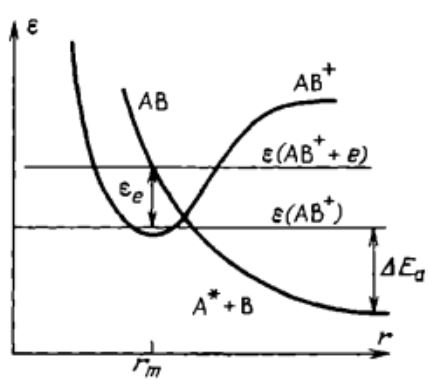
\includegraphics[width=70mm]{diss_recomb.JPG}}
	%\caption{\label{fig.2.4.2}}
\end{figure}
Первичным этапом диссоциативной рекомбинации является объединение молекулярного иона $АВ^{+}$ и электрона в квазимолекулу, которая находится в сверхвозбужденном автоионизационном состоянии. Соответствующая молекула $АВ$ может и не существовать, как в случае инертных газов, между атомами которых нет связи. Механизмом стабилизации захвата электрона ионом служит распад квазимолекулы на два атома; один из них может быть и возбужденным. Это возможно, если потенциальная кривая какого-либо из состояний системы атомов $А^{*} + В$ пересекает  потенциальную кривую иона $AB^{+}$. 
Системы $AB^{+} + e$ и $A^{*}+B$ при междуядерном расстоянии около $r_m$ имеют одинаковые энергии. Поэтому возможен самопроизвольный переход из первой конфигурации во вторую. 
Коэфициент диссоциативной рекомбинации равен:
\begin{equation}
\beta_{dis}=k_{capt}\frac{w_{stab}}{w_{stab}+w_{auto}}=\frac{k_{capt}}{w_{auto}}\frac{w_{stab}w_{auto}}{w_{stab}+w_{auto}}
\end{equation}
, где  $w_{auto} [c^{-1}]$- вероятность стабилизации (как и с излучением фотона - по факту обратное время жизни состояния) $w_{stab}\sim v_a[см/с] / a[см]$ скорость и размер частиц соответственно. Получается $w_{stab} \approx 10^{14} c^{-1}$, то есть это оч быстрый процесс. Он происходит даже быстрее, чем высвечивание кванта ($10^{8} c^{-1}$ )


\subsection{Прилипание.}
\label{sec.2.8}

 [райзер, стр. 145]
 
 
Процессы прилипания (attachment), сопровождающиеся образованием отрицательных ионов, важны для разрядов по двум причинам. Когда в тех газах, которые используются для исследований или приложений, имеются электроотрицательные компоненты, прилипание может играть заметную, иногда даже главную роль среди механизмов потерь электронов.
Они не зависят от механизмов образования и разрушения ионов и определяются уравнением Саха, в котором по смыслу роль положительных ионов играют нейтральные частицы, а роль атомов и молекул — отрицательные ионы:
\begin{equation}
	\frac{n_{-}}{n_e}=N\frac{g_{-}}{g_{a}}\frac{e^{I_{-}/kT}}{AT^{3/2}}
\end{equation}

\section{4. Динамика заряженных частиц в электрическом и магнитном полях}
\label{sec.4}

\subsection{Движение в скрещенных электрическом и магнитном полях.}
\label{sec.4.1}
(Ландау том 2(задачи) Котельник лекции)

Движение заряда в постоянном электрическом/магнтном или обоих полях: Ландау том2, параграфы 21-22(вроже это совсем 
примитивно, в конце есть задачи, хз будут ли это спрашивать).

\subsection{Дрейфовое приближение, разновидности дрейфового приближения.}
\label{sec.4.2}
Когда $\rho_H\ll l$, a $2\pi/\omega_B \ll \tau$, где $l$ - характерный масштаб изменения полей, a $\tau$ - характерное
время изменения полей, движение частицы можно разделить на быстрое вращение и медленное движение центра окружности.
Такое медленное движение называют дрейфом. Далее рассмотрим основные типы дрейфового движения.

\subsubsection{Электрический дреф}
\label{sec.4.2.1}
Запишем уравнение движения(пока для нерелятивизма):

\begin{equation}
    \begin{cases}
    \label{eq.4.2.1-motion}
        dr/dt = \upsilon \\
        dp/dt = e E + e/c [\upsilon \times B]
    \end{cases}
\end{equation}
легко видеть, что если перейти в систему, которая движется со скоростью $\upsilon_E = c\frac{E\times B}{B^2}$, то
уравнения движения примут вид:

\begin{equation}
    \begin{cases}
    \label{eq.4.2.2-motion}
    \dot{v_x}'=  \frac{eB}{mc} v'_y \\
    \dot{v_y}'= -\frac{eB}{mc} v'_x \\
    \dot{v_z}'=  \frac{e}{m} E_{\parallel}
    \end{cases}
\end{equation}
первые два уравенения дают движение по окружности, а третье - есть движение вдоль магнитного поля. В итоге в сопутствующей
системе отсчета (та, что со штрихом) имеем спираль. $\upsilon_E$ называют электрическим дрейфом, т.к. он вызван 
электрическим полем. По сути это дрейф нулевого порядка, тут поля постоянные и никаких неоднородностей нет. В плазме,
как правило, эта скорость мала по сравнению с тепловой, по этому этот дрейф отосят к первому порядку.
Также можно записать выражение для радиус-вектора ведущего центра (воображаемого центра дрейфующей системы). Есть два
способа это сделать:

\begin{equation}
    \label{eq.4.2.3-R1}
        \mathbf{R}'=\mathbf{r} + \frac{\mathbf{v}' \times \mathbf{B}}{\omega_H}
\end{equation}

\begin{equation}
    \label{eq.4.2.3-R2}
        \mathbf{R}=\mathbf{r} + \frac{\mathbf{v} \times \mathbf{B}}{\omega_H}
\end{equation}
В случае ~\ref{eq.4.2.3-R1} частица в сопутствующей с.о. заметает цилиндр (радиус ларморовской окружности постоянный), а
в случае ~\ref{eq.4.2.3-R2} будет гофрированная поверхность.

В релятивистском случае есть более общая офрмула для $\upsilon_E$, получаемая из преобразований Лоренца:

\begin{equation}
    \label{eq.4.2.4}
    \upsilon_E=c \frac{1-\sqrt{1-4\xi^2}}{2\xi^2} \frac{E \times B}{B^2 + E^2}
\end{equation}

где $\xi = |E\times B / (B^2 + E^2)|$. Легко видель, что, как с случае $E<B$, так и в обратном, это выражение дает 
скорость меньше скорости света. (???? $E=B$ ???).

\subsubsection{Дрейф под действем малой силы}
\label{sec.4.2.2}
В общем случае выражение для дрейфа получается из электрического заменой $e\mathbf{E}$ на $\mathbf{F}$:

\begin{equation}
    \label{eq.4.2.5}
    \upsilon_F=\frac{c}{e} \frac{\mathbf{F} \times \mathbf{B}}{B^2}
\end{equation}
также её можно получить усредняя уравнение движения $m\frac{d\mathbf{v}}{dt}=\mathbf{F} + \frac{e}{c} \mathbf{v}\times\mathbf{B}$
по периоду циклотронного вращения. Строго говоря, в уравнении~\ref{eq.4.2.5} стоит усредненная поперечная сила 
$\langle F_{\parallel} \rangle$, вила вдоль магниного поля дает нулевой вклад в дрейф. В случае, когда сила $F$ мала, есть
простой способ вычисления скорости дрейфа - надо усреднить по траектории(окружности), при остутствии силы $F$.

\subsubsection{Гравитационный дрейф}
\label{sec.4.2.3}

Пусть в качестве малой силы выступает гравитационная сила $m\mathbf{g}$. Скорость такого дрейфа 
$\upsilon_g=\frac{mc}{e} \frac{\mathbf{g}\times\mathbf{B}}{B^2}$ зависит от заряда частицы. Это вызывает ток в направлении $\upsilon_g$.

\subsubsection{Градиентный дрейф}
\label{sec.4.2.4}

Пусть электрического поля нет, а у магнитного есть градиент, перпендикутярный самому полю. Выполняя усреднение по
невозмущенной орбите легко получть: $\upsilon_{\nabla B}=\frac{v_{\perp}^2}{2\omega_B} \frac{\mathbf{B}\times\nabla_{perp}B }{B^2}$.

\subsubsection{Центробежный дрейф}
\label{sec.4.2.5}
В отстутствии внешней силы частица может иметь некоторую проекцию скорости на направление магнитного поля:
$\upsilon=v_{\parallel}  \frac{\mathbf{B}}{B}$, обозначим $\mathbf{h}= \mathbf{B}/B$. Если линии магнитного поля имеют некоторый
имеют некоторый изгиб, то на частицу будет действовать центробежная сила: $\mathbf{F}=-m\frac{d\upsilon}{dt}$. Распишем
производную от скорости:

\begin{equation}
    \label{eq.4.2.5-u}
    \frac{d\upsilon}{dt}=\frac{\partial \upsilon}{\partial t} + (\upsilon \nabla) \upsilon,
\end{equation}
где второе слагаемое есть движеие ведущего центра - это и есть центробежный дрейф, и выражение для скорости дрейфа:

\begin{equation}
    \label{eq.4.2.5-u}
    \upsilon_{cf} = -\frac{\mathbf{h}}{\omega_B} \times (\upsilon \nabla) \upsilon
\end{equation}
выражение для скорости можно упростить, если подставить выражения для скорости ведущего центра в нулевом порядке
и учесть, что в плазме $E/B \ll v/c$. Тогда выражение примет вид:

\begin{equation}
    \label{eq.4.2.5-u}
    \upsilon_{cf} = \frac{v_{\parallel}^2}{\omega_B} \mathbf{h} \times (\mathbf{h}\nabla)\mathbf{h},
\end{equation}
эта скорость направлена по бинормали магнитной линни и зависит от знака заряда.

\subsubsection{Поляризационный дрейф}
\label{sec.4.2.6}

Первое слагаемое в выражении~\ref{eq.4.2.5-u} отвечает за поляризоционый дрейф.

\begin{equation}
    \label{eq.4.2.5-u}
    \upsilon_{pol} = \frac{\mathbf{h}}{\omega_B} \times \frac{\partial \upsilon}{\partial t},
\end{equation}
далее подставляя выражение для скорости ведущего центра и учитывая, что электрическое поле близко к потенциальному
можно получить:

\begin{equation}
    \label{eq.4.2.5-u}
    \upsilon_{pol} = \frac{c}{B\omega_B} \frac{\partial \mathbf{E}_{\perp}}{\partial t},
\end{equation}
она зависит от заряда, по этому в переменном поле плазма поляризуется. Поскольку плазма это проводник, постояную
поляризацию разделеными зарядами создать нельзя, но когда есть переменное электрическое поле, возникает переменный 
поляризационный ток и он вызывает реальную поляризацию плазмы.

\subsubsection{Дрейф в неоднородном электрическом поле}
\label{sec.4.2.7}
Аналогично магнитному полу, получаем для скорости дрейфа:

\begin{equation}
    \label{eq.4.2.5-u}
    \upsilon_{\nabla E} = \frac{c\rho_B^2}{4 B^2} \nabla^2_{\perp}\mathbf{E}\times \mathbf{B},
\end{equation}
она зависит от заряда, и создает ток, это т.н. эффект конечного ларморовского радиуса.

\subsection{Заряженная частица в высокочастотном поле}
\label{sec.4.3}
(тут только нерелятовистский случай)

Пусть есть в.ч. поле: $\mathbf{E}=Re\mathbf{E}(\mathbf{r}\exp(-i\omega t), \mathbf{B}=Re\mathbf{B}(\mathbf{r}\exp(-i\omega t)$, где $\mathbf{E}(\mathbf{r}), \mathbf{B}(\mathbf{r})$ медленно меняющиеся амплитуды (по сравнению с характерым
ларморовским радиусом). Тогда движенеи разбивается на медленный дрейф и быстрые осцилляции: $\mathbf{r}=\mathbf{R}+\mathbf{\rho}$. 
Тогда разложим электрическое поле(магнитное убираем, т.к. нерелятивизм): $E(\mathbf{r})=E(\mathbf{R})+(\mathbf{\rho} \nabla)E(\mathbf{R})$. В нулевом приближении мы принебрегаем вторым членом и уравнение движения в первом порядке имеет 
следующий вид(? $\mathbf{R}$ убираем т.к. меняется слабо?):

\begin{equation}
    \label{eq.4.3-0}
    \ddot{\mathbf{\rho}}=\mathbf{E}(\mathbf{R}) \frac{e}{m} \exp(-i\omega t).
\end{equation}
В следующем поярдке усредним по периоду $2\pi/\omega$ радиус вектор ($\rho$ уйдет, т.к. в среднем 0):

\begin{equation}
    \label{eq.4.3-1}
    \ddot{\mathbf{R}}=-\frac{-e^2}{m^2 \omega^2}\langle \mathbf{E} \exp(-i\omega t) \nabla \mathbf{E} \exp(-i\omega t) \rangle, 
\end{equation}
подставляя сюда выражение~\ref{eq.4.3-0}, получаем выражение для пондермоторного силы:

\begin{equation}
    \label{eq.4.3pf}
    \ddot{\mathbf{R}}=-\frac{-e^2}{4 m^2 \omega^2} \nabla |E|^2.
\end{equation}
(что еще тут ?)

\subsection{Понятие адиабатического инварианта}
\label{sec.4.4}

\subsubsection{Понятие адиабатического инварианта}
\label{sec.4.4.1}
Площадь потока матнитного поля $\Upphi=\pi \rho B$ через ларморовскую окружность в сопутствующей системе является
адиабатическим инвариантом - приближенно сохраняется при медленном изменении полей. Постоянство следует из закона
Фарадея: $\mathcal{E}=-\dot{\Upphi}/c$, где по законе Ома $\mathcal{E}=IR=0$, т.к. сопративления нет т.к. принебрегаем
столкновениями.

Для случая частицы движузейся в однородных электрическом и магнитных полях, в общем случае адиабат. инвариант есть:

\begin{equation}
    \label{eq.4.3pf}
    J_{\perp} = \frac{1}{2\pi} \oint \mathbf{P}_{\perp} d\mathbf{r}_{\perp},
\end{equation}
где интеграл берется по пероду вращения частицы в с.с.о. Далее используя теорему Стокса можно получить, что:

\begin{equation}
    \label{eq.4.3pf}
    J_{\perp} = \frac{m\upsilon_{\perp}^2}{2\omega_B}=\frac{|e|}{2\pi c} \Upphi, 
\end{equation}
В общем случае адиабат. нвариантам являются следующие величины: $\Upphi$, $\gamma \mu$, $p_{\perp}^2/B$.

\subsubsection{Продольный адиабатический инвариант}
\label{sec.4.4.2}
В магнитных пробках, в нулевом приближении частица движется вдоль силовой линии от поворота к повороту. Интеграл вдоль
такого движения есть т.н. продольный адиабат. инвариант:

\begin{equation}
    \label{eq.4.3pf}
    J_{\parallel} = \frac{1}{2\pi}\oint\mathbf{P}_{\parallel}ds=1/\pi \int \sqrt{2m \left(\varepsilon - e\phi - \mu B - 0.5m\upsilon_E^2 \right)}. 
\end{equation}
Этот интеграл зависит от следующих параметров $J_{\parallel}=J_{\parallel}(x_0, y_0, \varepsilon, \mu)$, где $x_0, y_0$
есть координаты пересечения силовой линии с поверхностью рассекающую магнитную ловушку поперек.

\subsubsection{Третий адиабатический инвариант}
\label{sec.4.4.3}

В магнитной ловушке частица движется от одного конца к другому, смещаясь вдоль экватора, заметая некую поверхность - 
дрейфовую оболочку. Если магнитное поле и потенциал медленно меняются, сохраняется магнитный поток через сечение 
дрейфовой оболочки:

\begin{equation}
    \label{eq.4.3pf}
     \Upphi_{dr}= \int_{S_{dr}} \mathbf{B}d\mathbf{S}.
\end{equation}

Эти адиабат. инварианты удобны для нахождения завичимости энергии частицы от времени.


\section{ 7.Колебания и волны в плазме}
\label{sec.7}

\subsection{Основные типы колебания и волн в плазме: лэнгмюровские электонные и ионные, электромагнитные, ионно-звуковые, магнитозвуковые, альфвеновские.}
\label{sec.7.1}

В изотропной плазме легко записат дисперсионное уравнение:

\begin{equation}
    \label{eq.7.1}
    \left(1-\frac{\omega^2}{c^2 k^2} \varepsilon_{\perp}\right) E_{\perp} + \varepsilon_{\parallel} E_{\parallel}= 0
\end{equation}

Отсюда, при условии $\varepsilon_{\parallel} = 0$ получаем первый тип волн - продольные(ленгмюровские/электростатические) 
волны. Затухание Ландау(безстолкновительное затухание) относится именно к таким волнам. Их дисперсионка имеет следующий
вид:

\begin{equation}
    \label{eq.7.2}
    \omega^2=\omega_p^2 + 3/2 (k v_{t})^2
\end{equation}
волны с частотой сильно отличной от плазменное затухают.

В случае $1 - \frac{\omega^2}{c^2 k^2} \varepsilon_{\parallel}=0$ получаем поперечные волны(почти как в вакууме). Для них
дисперсионка:

\begin{equation}
    \label{eq.7.3}
    \omega^2=\omega_p^2 + (c k)^2
\end{equation}
Легко видеть, что волны с частотой $\omega < \omega_p$ не распространяются.

Если еще учесть ионы:

\begin{equation}
    \label{eq.7.4}
    \varepsilon=1+\frac{\omega_{pe}^2}{k^2 v_{Te}^2} - \frac{\omega_{pi}^2}{\omega^2}-3\frac{\omega_{pi}^2 k^2 v_{Ti}^2}{\omega^4}
\end{equation}
В случае низких частот(где влияние ионов существенно) можно принебреч 4ым слашаемым, тогда дисперсионка примет следующий вид:

\begin{equation}
    \label{eq.7.5}
    \omega=\frac{k c_s}{\sqrt{1 + k^2 r_d^2}}
\end{equation}
при малых $k$ имеем $\omega=k c_s$, где $c_s=\frac{T_i + T_e}{M}$ (ионный звук). При больших частотах имеем ионные ленгмюровские волны (сильно затухают, если температура ионов не мала). Грубо дисперсионные соотношения для разных волн изоражены на рисунке~\ref{plot.7.1}.

\begin{figure}[h!]
    \center{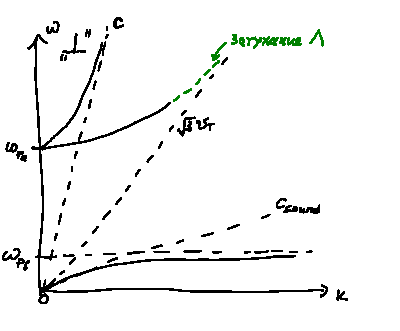
\includegraphics[width=85mm]{noB.pdf}}
    \caption{\label{plot.7.1} Дисперсионка для волн в плазме в отсутствии магнитного поля.}
\end{figure}

Магнитоактивная плазма

Пусть есть внешнее магнитное поле $B_0$, будем рассматривать холодную плазму. Вводя обозначения $n^2=\frac{c^2 k^2}{\omega^2}$, $\upsilon=\frac{\omega_p^2}{\omega^2}$, $u=\frac{\omega_H^2}{\omega^2}$, где $\omega_H$ - циклотронная частота,
дисперсионку можно записать следующим образом:

\begin{equation}
    \label{eq.7.6}
    n_{e,o}^2=1-\frac{2\upsilon (1-\upsilon)}{2(1-\upsilon) - u \sin^2(\theta) \pm \sqrt{u^2 \sin^4(\theta) + 4u(1-\upsilon)^2 \cos^2(\theta)}}, 
\end{equation}
где $\theta$ это угол между магнитным полем и волновым вектором. Индексы e,o соответствуют необыкновенной и обыкновенной волнам.
Cлучай $\theta=0$ представлен на графиках \ref{theta0-u-less-1, theta0-u-more-1}, важно обратить внимание на то, что формула~\ref{eq.7.6} не дает полного решения, нужно ещё учесть $\varepsilon_{\parallel}=0$.

\begin{figure}[h!]
    \center{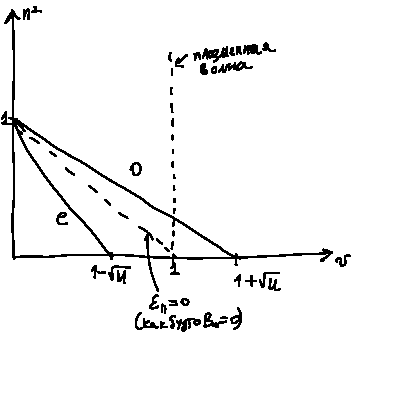
\includegraphics[width=85mm]{theta0-u-less-1.pdf}}
    \caption{\label{theta0-u-less-1} Случай $\theta=0, u < 1$.}
\end{figure}

\begin{figure}[h!]
    \center{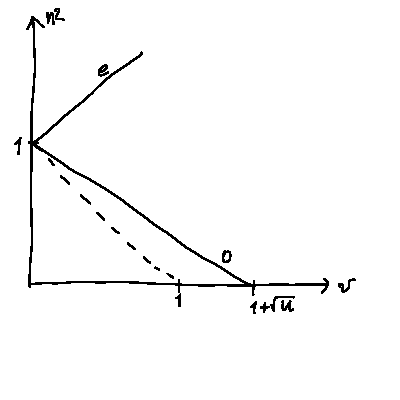
\includegraphics[width=85mm]{theta0-u-more-1.pdf}}
    \caption{\label{theta0-u-more-1} Случай $\theta=0, u > 1$.}
\end{figure}

Теперь расмотрим случай $\theta \ll 1$ (предельного перехода между $\theta=0$ и $\theta \neq 0$, при отсутствии
теплового движения и столкновений нет), дисперсионка в этом случае изображена на рис.~\ref{theta-small-u-less-1, theta-small-u-more-1}. При наличии необнородностей в областях сближения одна волна может переходить в другую.
\begin{figure}[h!]
    \center{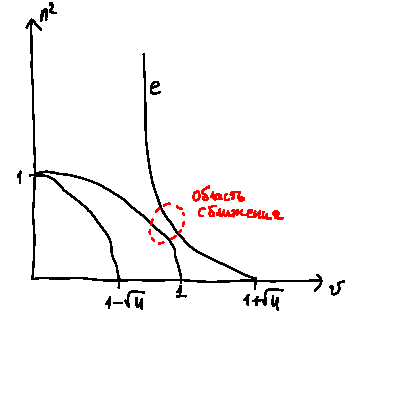
\includegraphics[width=85mm]{theta-small-u-less-1.pdf}}
    \caption{\label{theta-small-u-less-1} Случай $\theta\ll1, u < 1$.}
\end{figure}

\begin{figure}[h!]
    \center{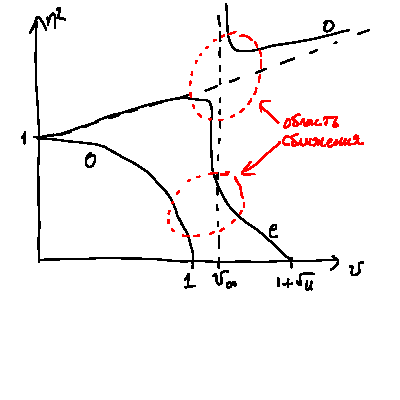
\includegraphics[width=85mm]{theta-small-u-more-1.pdf}}
    \caption{\label{theta-small-u-more-1} Случай $\theta\ll1, u < 1$.}
\end{figure}

Когда $\theta=\pi/2$ график дисперсионка имеет следующий вид~\ref{theta90}.
\begin{figure}[h!]
    \center{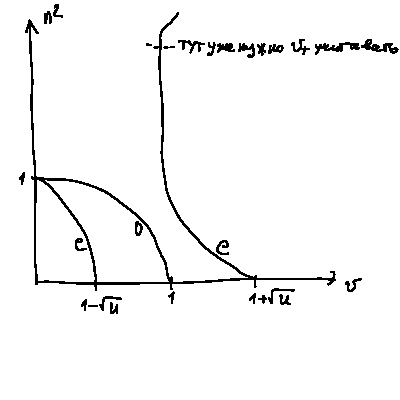
\includegraphics[width=85mm]{theta-90.pdf}}
    \caption{\label{theta-90} Случай $\theta=\pi/2$.}
\end{figure}

Альфвеновские волны. При рассмотрении предыдущих волн, движением ионов принебрегалось. Рассматриваем случай, когда волна распространяется вдоль вшеншего магнитного поля; также рассматриваются низкие частоты (сравнимые с циклотронной частотой ионов ?). Дисперсионка таких волн имеет следующий вид:

\begin{equation}
    \label{alfven}
    \frac{\omega}{k}=\frac{B_0}{\sqrt{4\pi \rho}}
\end{equation}
где $\rho$ есть масстовая плотнотсь плазмы (все частицы). Важно, что фазовая скорость не зависит от частоты! По сути это совместное движение/осцилляции ионов и магных силовых линий поперек движения волны. Они распространяются без дисперсии.

\subsection{Показатель преломления плазмы, пространственная и временная дисперсии, фазовая и групповая скорости плазменных волн.}
\label{sec.7.2}


Диэлектрическая проницаемость в холодной плазме с учетом ионов:

\begin{equation}
    \label{eq.7.7}
    \varepsilon=1 - \frac{\omega_{pe}^2}{\omega^2} - \frac{\omega_{pi}^2}{\omega^2},
\end{equation}
если есть столкновения (пусть отбросим ионы), то $\varepsilon=1-\frac{\omega_{pe}^2}{\omega (\omega+i \nu)}$. когда есть некоторый поток, движущийся со скоростью $\upsilon_0$, то без учета ионов и столкновений, имеем: $\varepsilon=1-\frac{\omega_{pe}^2}{(\omega - k \upsilon_0)^2}$.
Для затухания Ландау: $\varepsilon=1+\frac{4\pi e^2}{m} \int \frac{v}{\omega} \frac{\partial f_0}{\partial v} \frac{dv}{\omega-vk}$.

При наличии внешнего магнитного поля $B_0$ диэликтрическая проницаемость перестает быть изотропной(считаем, что трения нет и $\upsilon_T \ll \upsilon_{ph}$):

\begin{equation}
    \label{eq.7.8}
    \varepsilon=
    \begin{pmatrix}
        \varepsilon_B & ig & 0 \\
        -ig & \varepsilon_B & 0 \\
        0 & 0 & \varepsilon_{\parallel}
    \end{pmatrix}
\end{equation}
 где $\varepsilon_B=1-\frac{\omega_{pe}^2}{\omega^2-\omega_{Be}^2}-\frac{\omega_{pi}^2}{\omega^2-\omega_{Bi^2}}$ и $g=\frac{\omega_{pe}^2 \omega_{Be}}{\omega (\omega^2-\omega_{Be}^2} -\frac{\omega_{pe}^2 \omega_{Be}}{\omega (\omega^2-\omega_{Be}^2}$, $\varepsilon_{\parallel}=1-\frac{\omega_{pe}^2}{\omega^2}-\frac{\omega_{pe}^2}{\omega^2}$. 

Фазовые и групповые скорость изображениы на графиках~\ref{noB} и т.д. Из необычного - фазовая скорость всегда больше скорости света(но это не страшно). 

Пространственная и временная дисперсия(??? общие вещи):
В общем случаем имеем:
\begin{equation}
    \label{eq.7.8}
    \overrightarrow{D}=\iint \varepsilon(t,t',\overrightarrow{r},\overrightarrow{r}') \overrightarrow{E}(t',\overrightarrow{r}') d^3 r' dt,
\end{equation}
в случае однородной и стационарной среды имеем $\varepsilon(t-t', \overrightarrow{r}-\overrightarrow{r}')$, в этом случае
также справедливо $\varepsilon(\omega, \overrightarrow{k})= \varepsilon^*(-\omega, -\overrightarrow{k})$.

\section{Прикладные проблемы физики плазмы}
\label{sec.14}


\subsection{Управляемый термоядерный синтез}
\label{14}

[Кенро Миямото, Основы Физики Плазмы и управляемого термоядерного синтеза, Москва, физматлит 2007]

Всем известно про дефект масс, что при слиянии ядер до Fe и Ni выделяется энергия.
основная реакция D+T-> 4He + n [17.59 MeV], 1/5 энергии приходится на He и 4/5 на n
Чтобы сблизить ядра на достаточное расстояние надо преодолеть кулоновский барьер. ту силу, с которой они отталкиваются ($Z_{alpha}Z_p e^2/r_N$) вычислили, что примерное расстояние $r_{n}=1.4*10^{-13}*(A^{1/3}_{\alpha}+A^{1/3}_{\beta}) [cm]$ Но это оказалось слишком мало, ибо не сходилось с вычислениями T солнца, для 10кэВ вычислили точку остановки $R_t=10^{-11} [cm]$

[Миямото стр. 23]

Почему вообще надо удерживать плазму, какие характерные времена? Критерий Лоунсена 
Дело обстоит в том, что система должна сама себя поддерживать и при этом отдавать эл. энергию. Энергия в единице объёма $(3/2)nk(T_i+T_e)$. Время остывания $\tau_E = \frac { (3/2)nk(T_i+T_e) }{P_L+R}$, , где $P_L$ и $R$ соответственно мощность потерь энергии на диффузию и излучение плазмой. В то же время, в объёме происходит выделение тепла за счёт термоядерного синтеза мощностью. $P_{NF}=(n/2)(n/2)<\sigma v> Q_{NF} $. Потому
 как D и T присутствуют в реакторе в равном количестве и концентрация каждого n/2 соответственно. $<\sigma v> $ - вероятность процесса,   $Q_{NF} $ энергия на одну реакцию.
Чтобы всё было устойчиво и не затухало: $P_{heat}=P_L + R = \frac{3nkT}{\tau_E} < \eta_{el} \eta_{heat} P_{NF} $, где $\eta_{el} $ - КПД получения эл. мощности ,$ \eta_{heat} $ - КПД нагрева.

Итого: $ \frac{3nkT}{\tau_E} < \eta_{el} \eta_{heat} Q_{NF} n^{2} \frac{<\sigma v>}{4}$

\begin{equation}
	\label{eq.Disp14.1.1}
	n \tau_E > \frac{12 kT}{\eta Q_{NF} <\sigma v>} > 1.7*10^{20} m^{-3} s
\end{equation}
 - Критерий Лоунсена , критерий термоядерности. То есть надо или увеличивать концентрацию, или время удержания. Поэтому есть как токамаки с непрерывным временем работы, так и импульсные(импульсно поддерживается магнитное поле).
Понятно, что чем горячее плазма, тем труднее её удерживать, понятно что удерживать надо именно магнитным полем.

\subsection{Магнитное удержание}
\label{14.1}

Уравнения магнитной гидродинамики тут написаны [Голант Жилинский Сахаров, Основы ФП,  §10.1]

Из уравнения для средней скорости $\rho (du/dt)=(1/c)[j H]-grad\;p$; где $p=p_e+p_i$ - суммарное давление, $j=en(u_i+u_e)$ - плотность тока, $ du/dt=\delta u / \delta t + (u grad)u$ полная производная

можно вывести условие равновесия
\begin{equation}
	\label{eq.Disp14.1.2}
	\frac{1}{c}[j H]=grad\;p
\end{equation}
[Голант Жилинский Сахаров, Основы ФП,  §10.2]


Идея состоит в том, что преодолеть давление плазмы как газа с ооочень большой температурой с помощью давления магнитного поля около стенок.
Первая задача, возникающая при рассмотрении удержания плазмы в магнитном поле, заключается в определении условий, при которых достигается равновесие, т. е. электродинамические силы, действующие на каждый элемент объема плазмы, уравновешивают градиент давления.
\begin{equation}
	\label{eq.Disp14.1.3}
	G_H=\frac{1}{c} [j H]=\frac{1}{4 \pi} [H rotH]=-\frac{1}{8 \pi} grad(H^{2})+\frac{1}{4 \pi} (H grad) H
\end{equation}
Так же есть отдельный случай, когда линии имеют радиус кривизны R.

\begin{equation}
	\label{eq.Disp14.1.4}
(\vec H grad)\vec H=H(\vec h grad)\vec h H=H^{2} grad_{||}\vec h + \frac{1}{2} grad_{||} H^{2}=-H^{2} \frac{\vec R}{R}+\frac{1}{2} grad_{||} H^{2}
\end{equation}


, где $\vec h= \frac{\vec H}{H}$; $grad_{||}=(\vec h \; grad)$ - проекция градиента на направление магнитного поля. Подставляем в предыдущее выражение и получаем, что давление:
\begin{equation}
	\label{eq.Disp14.1.5}
 G_H=-grad_{\perp}(H^{2}/8\pi)-(H^{2}/4\pi R^{2})\vec R
\end{equation}
Первое слагаемое в представляет собой поперечный градиент введённого магнитного давления. Действие этой силы можно описать как взаимное «расталкивание» силовых линий в поперечном направлении. Второе слагаемое определяет силу, направленную к центру кривизны силовых линий, и называется натяжением магнитного поля. Оно формально получается, если приписать силовым линиям свойства растянутой струны.

Для равновесия: 
\begin{equation}
	\label{eq.Disp14.1.6}
 grad p + grad_{\perp}(H^{2}/8\pi)+(H^{2}/4\pi R^{2})\vec R =0
\end{equation}

Для случая, когда силовые линии прямые ($R\rightarrow \inf $), уравнение сводится к постоянству суммы кинетического и магнитного давлений в плоскости, перпендикулярной магнитному полю:
\begin{equation}
	\label{eq.Disp14.1.7}
p + H^{2}/8\pi=const
\end{equation}
\begin{equation}
	\label{eq.Disp14.1.8}
p_0 + H_{0}^{2}/8\pi=H_{e}^{2}/8\pi
\end{equation}

Равенство показывает, что максимальное давление плазмы, которое можно удерживать магнитным полем, равно магнитному давлению вне плазмы $H_{e}^{2}/8\pi$. При описании магнитного удержания часто вводят коэффициент $\beta$, представляющий собой
отношение давления удерживаемой плазмы к максимально возможному: $\beta=p/p_{max}=8\pi p/H_{e}^{2}$
Но это удержание поперёк линий магнитного поля, а строить комплексы в виде торов не всегда удобно, поэтому было придумано пробочное удержание.

пробочное удержание [Миямото стр. 32]

Понятно, что всё движение электрона в магнитном поле можно описать как движение вдоль и поперёк поля. Вдоль - свободное движение, поперёк - ларморовское вращение.
Если рассмотрим электрон в поле, он будет вращаться по кругу с радиусом равному Ларморовскому. Его можно представить в виде витка с током. У витка с током есть магнитный момент.
\begin{equation}
	\label{eq.Disp14.1.9}
 \mu=I*S=\frac{q\Omega}{2\pi} * \pi \frac{\rho^{2}}{2}=\frac{mv_{perp}^{2}}{2B}
\end{equation}	
Но кин энергия должна сохранятся при движении в магнитном поле, поэтому электрон будет лететь вдоль поля пока
\begin{equation}
	\label{eq.Disp14.1.10}
	\frac{mv_{||}^{2}}{2}+\frac{mv_{\perp}^{2}}{2}=\frac{mv^{2}}{2}=const
\end{equation}	
Поскольку магнитный момент сохраняется, то:
\begin{equation}
	\label{eq.Disp14.1.11}
 v_{||}=+-(\frac{2}{m}E-v_{\perp}^{2})^{1/2}=+-(v^{2}-\frac{2}{m} \mu B)^{1/2}
\end{equation}	
То есть электрон может полностью убрать продольную скорость и отразиться. Почему возникает этот эффект ? Потому что на магнитный диполь действует сила $-\mu \grad_{||}$ B. Ну и вводится пробочное отношение - отношение магнитных полей в центре и на краях ловушки $R_M=\frac{B_M}{B_0}$


\subsection{Плазменные источники излучения}
\label{14.4} 
раз­дел фи­зи­ки плаз­мы, изу­чаю­щий кол­лек­тив­ные взаи­мо­дей­ст­вия плот­ных по­то­ков (пуч­ков) за­ря­жен­ных час­тиц с плаз­мой и га­зом, при­во­дя­щие к воз­бу­ж­де­нию в сис­те­ме ли­ней­ных и не­ли­ней­ных элек­тро­маг­нит­ных волн и ко­ле­ба­ний, и ис­поль­зо­ва­ние эф­фек­тов та­ко­го взаи­мо­дей­ст­вия.
плаз­мен­ные ус­ко­ри­те­ли, ос­но­ван­ные на яв­ле­нии кол­лек­тив­но­го ус­ко­ре­ния тя­жё­лых за­ря­жен­ных час­тиц элек­трон­ны­ми пуч­ка­ми и вол­на­ми в плаз­ме

плаз­мен­но-пуч­ко­вый раз­ряд, ос­но­ван­ный на кол­лек­тив­ном ме­ха­низ­ме взаи­мо­дей­ст­вия плот­ных пуч­ков за­ря­жен­ных час­тиц с га­зом;

тур­бу­лент­ный на­грев плаз­мы плот­ны­ми пуч­ка­ми за­ря­жен­ных час­тиц и кол­лек­тив­ные про­цес­сы при транс­пор­ти­ров­ке и фо­ку­си­ров­ке пуч­ков в про­бле­ме управ­ляе­мо­го тер­мо­ядер­но­го син­те­за (УТС);

[Богданкевич Л С, Кузелев М В, Рухадзе А А "Плазменная СВЧ электроника" УФН 133 3–32 (1981)]
DOI: 10.3367/UFNr.0133.198101a.0003
URL: https://ufn.ru/ru/articles/1981/1/a/

Когда говорят о сильноточных электронных пучках, то прежде всего имеют в виду пучки с током, превышающим так называемый предельный вакуумный ток. Известно, что в металлическом волноводе с радиусом R и длиной $L >> R$, который обычно используется в вакуумной электронике в качестве резонатора, ток пучка ограничен пространственным зарядом электронов, причем предельный ток по порядку величины определяется соотношением:
\begin{equation}
	\omega_{b \; vol}^{2} \approx \frac{c^{2}}{S} \gamma
\end{equation}
, где $\gamma = [1-(u^{2}/c^{2})]^{-1/2}$ - — релятивистский фактор энергии электронов, $S$ — поперечное сечение пучка, меньшее или порядка сечения волновода, а $\omega_{b}=\sqrt{4\pi e^{2} n_{b} /m}$ — лэнгмюровская частота электронов пучка. 


Следовательно, сильноточным следует считать пучок, в котором $\omega_{b}^{2}>\omega_{b\;vol}^{2}$. Такой пучок может распространяться в волноводе только при наличии нейтрализации пространственного заряда электронов, что достигается заполнением системы относительно плотной (по сравнению с плотностью пучка) плазмой. Таким образом, сильноточная СВЧ электроника, строго говоря, может быть только плазменной. При этом, однако, плазма может и не влиять существенным образом на частоты генерируемых пучком электромагнитных волн. Дело в том, что длины волн возбуждаемых пучком электромагнитных колебаний меньше или порядка поперечных размеров электродинамической системы генератора, т. е. резонатора, точнее $\omega>\omega_{crit}= \mu c/R$, где $\mu$ характеризует радиальное волновое число моды колебаний (корни функций Бесселя или ее производных); обычно $\mu \sim 3-10$. Если плазма, заполняющая резонатор, имеет относительно низкую плотность, так что $\omega_{pl}=\sqrt{4\pi e^{2} n_{p} /m} < \mu c/R$ , то она существенно не меняет электродинамику резонатора, который по своим электродинамическим свойствам остается практически вакуумным. Вместе с тем такая плазма может нейтрализовать пространственный заряд пучка и позволить пропустить через резонатор сильноточный пучок со сверхпредельным током. Однако ток пучка при этом ненамного может превышать предельный, не более, чем в $\mu^{2} S/\gamma R^{2}$ раз, что следует из неравенств $\omega_{b}^{2}<\omega_{p}^{2}<\mu^{2} c^{2}/R^{2}$.

Иное положение имеет место в случае достаточно плотной плазмы, когда $\omega_{pl}>\mu c/R$. Роль такой плазмы в резонаторе не ограничивается нейтрализацией пространственного заряда пучка, она существенно меняет всю электродинамику резонатора и, в частности, спектры частот собственных электромагнитных мод резонатора. Именно в этом случае мы имеем дело с настоящей плазменной электроникой, которая, как будет видно из дальнейшего, позволяет продвинуться в область токов электронного пучка, намного превосходящих предельный вакуумный ток, вплоть до $\mu^{2}\gamma S/R^{2}$ раз. Более того, с помощью ультрарелятивистских электронных пучков в таких системах оказывается возможным эффективное возбуждение колебаний с длиной волны, намного меньшей поперечных размеров резонатора $\lambda \approx R/\gamma^{2}$ .

\begin{figure}[h!]
	\center{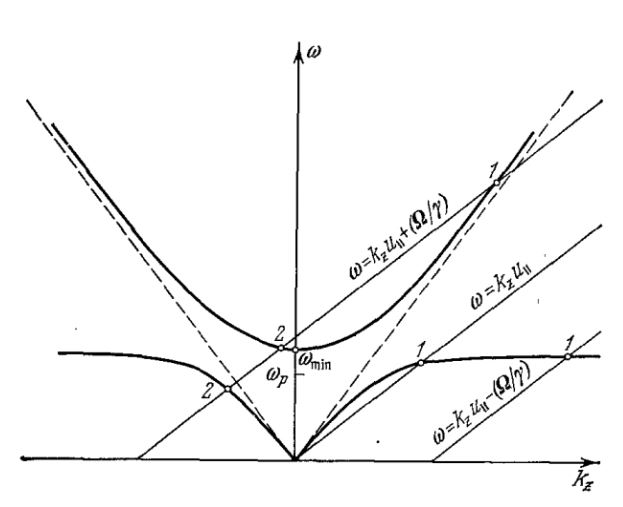
\includegraphics[width=70mm]{dispers_14_3.JPG}}
	%\caption{\label{fig.2.4.1}}
\end{figure}

Другими словами, плазменная СВЧ электроника открывает возможиость создания коротковолновых источников мощного электромагнитного излучения.


Без формул, наверное сразу можно нарисовать дисперсионку резонатора, без пучка.  Как мы видим при добвалении плазмы, появилась ещё одна нижняя ветвь. Точки 1. это работа в режиме усилителя. Пучок (наклонные линии $\omega=ku\pm (\Omega/\gamma)$) усиливает волну бегущую в ту же сторону. Точки 2. это работа в режиме генератора. Пучок усиливает встречную волну.



плазменная СВЧ электроника.
Компрессоры импульсов.


\subsection{Преобразование тепловой энергии в электрическую: МГД-преобразователи, тепловые преобразователи}
\label{14.5} 
[райзер, дополнение, стр. 673]

\begin{figure}[h!]
	\center{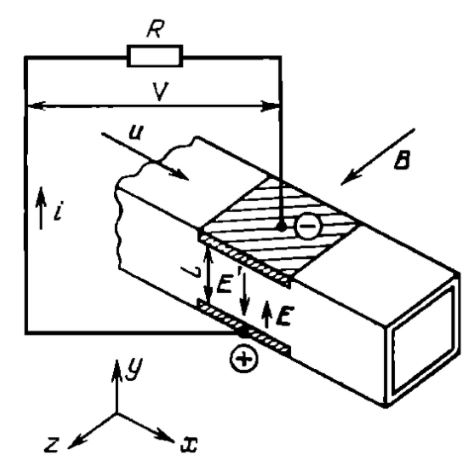
\includegraphics[width=70mm]{MGD_generator.JPG}}
	%\caption{\label{fig.2.4.1}}
\end{figure}

Принцип работы МГД генератора представлен на рисунке. Ионизованный газ протекает по каналу со скоростью и и пересекает линии напряженности приложенного постоянного магнитного поля. В движущейся среде индуцируется электрическое поле $Е' =\frac{1}{c} [V\; В]$. Вектор магнитной индукции $В =\mu H$ не отличается от $Н$, поскольку магнитная проницаемость газа $\mu=1$. Направление Е' характеризуется  
координатным равенством $E’_y=-u_x B_z / c $. Индуцированное поле Е' движет электроны вверх. У верхней  
стенки канала накапливается отрицательный пространственный заряд, у нижней — положительный. Если внешняя цепь между электродами, помещенными на этих стенках, разомкнута, заряды накапливаются, пока созданное ими электрическое поле $E_{\inf}$ не уничтожит индуцированное ($E_{\inf}=-E’$). Потенциал нижнего электрода при этом превышает потенциал верхнего на $V_{\inf} = E_{inf} L$. Это напряжение совпадает по величине с ЭДС генератора:
\begin{equation}
	\varepsilon=E’_{y}L=(-u_x /c)(B_z L)
\end{equation}

Если цепь замкнуть через нагрузочное сопротивление и обеспечить достаточно высокую электронную эмиссию с нижнего электрода, например путем его активирования и нагревания, в цепи потечет ток. Реально электроны в газе непрерывным потоком дрейфуют вверх, исходя из нижнего положительного электрода, который в отличие от обычного разряда работает подобно катоду, и внедряясь в верхний. Частичное устранение приэлектродного пространственного заряда, уносимого током, приводит к уменьшению напряжения на электродах $V= Е_{y} L$ по сравнению с $V_{inf}=|\varepsilon|$. В пренебрежении эффектом Холла, в результате которого возникает ток по оси $х \perp Е, В$, плотность тока в газе:
\begin{equation}
	j=\sigma(E+E’)=\sigma(E+\frac{1}{c}[u\;B])
\end{equation}

Ну или в нашей системе координат 
\begin{equation}
	j_y=\sigma(E_y-\frac{[u\;B]}{c}) <0
\end{equation}

Дело ещё обстоит в том, что ток в цепи как раз и зависит от E меж электрожного промежутка, как $i*R=V$ (общий ток через систему с площадью $S$, $i=j*S$), в то время как $V=E*L$, то есть мы получили систему самосогласованных уравнений, которые замкнулись сами на себя. А именно:
\begin{equation}
	i=S \sigma(V/L-uB/c)=S \sigma(iR/L-uB/c)
\end{equation}
отсюда можно выразить $i$ в чистом виде. $i=\frac{u\;B}{c(\frac{R}{L}-\frac{1}{\sigma S})}$

При протекании тока на газ действует тормозящая пондеромоторная сила, в результате чего он и теряет энергию. Отношение мощности, выделяемой в нагрузке, к мощности, отбираемой от газа: 
\begin{equation}
	\frac{iV}{(u/c)(jB)LS}=\frac{V}{\varepsilon}
\end{equation}

т. е. электрический КПД генератора тем выше, чем ближе ситуация к режиму разомкнутой цепи. Но абсолютное значение полезной мощности $iV$ максимально, когда сопротивления нагрузки и плазмы одинаковы и $V=|\varepsilon|/2$


\subsection{Химические реакции в равновесной и неравновесной плазме. \textcolor[rgb]{1,0,0}{Механизмы и кинетика осуществления плазмохимических реакций, роль заряженных и возбужденных частиц. Энергетика химических реакций в электрических разрядах}. Закалка продуктов плазмохимических процессов.}

\label{14.6}

 
[В.Д. Русанов, А.А. Фридман, Физика химически-активной плазмы]

Очевидно, что хотели увеличить скорость некоторых процессов и сократить их количество. Поэтому некоторые реакции хотели провести напрямую в плазме. В рамках классической кинетики при этом экспоненциально ускоряется в соответствии с известным законом Аррениуса $ к \sim exp(-E_{a}/T)$, где $E_a$ — характерная величина энергетического барьера реакции; Т — температура системы. (Понятно, что хим реакция протекает при столкновении двух/трёх частиц, каждая из которых может быть подчинена максвеллу).
 
Резкое повышение скорости процесса может иметь место уже при температурах 3000—5000° С, что значительно выше обычного диапазона температур химических, технологических и  металлургических процессов. Скорость переноса реагентов через зону реакции, очевидно, должна соответствовать повышенной удельной производительности, которая достигается в реакционной зоне при очень высоких температурах, что можно реализовать только в случае газового транспорта реагентов с повышенными скоростями ($5*10^{3}—5*10^{4}$ см/с). 
Очевидно, что подвод к газу столь высокопотенциального тепла не может быть осуществлен с помощью традиционных методов теплопередачи. Сверхвысокие температуры в реакционной зоне должны обеспечиваться подводом энергии электромагнитного поля от внешнего источника, а не тепловой энергии. Этим требованиям отвечает совмещение реакционной зоны с газоразрядной, в которой можно организовать локальный нагрев реагентов до высоких температур за счет активных потерь энергии электромагнитного поля.

Плазмохимические системы в целом можно условно разделить на два больших класса — квазиравновесные и неравновесные.
Температура Т в случае, когда система близка к равновесию (квазиравновесию), является единственной энергетической характеристикой системы, т. е. $Т \approx T_{o} \approx Т_{e} \approx T_{i} \approx  Т_{r} = T_{v}$, где $Т_{o}$ — поступательная температура нейтрального газа, $Т_e$ — температура электронов; $Т_i$ — температура ионов; $Т_r$ — вращательная температура молекул; $T_v$— колебательная температура молекулярного газа. 

Если равновесие в системе не достигнуто, то могут реализоваться различные неравновесные (неизотермические) ситуации, из которых наибольший практический интерес с точки зрения оптимизации характеристик реакционной зоны имеют простейшие системы 

\begin{equation}
T_e \textgreater T_0, T_i, T_v,T_r
\end{equation}

\begin{equation}
T_e \textgreater T_i \textgreater T_0  \approx T_v  \approx T_r
\end{equation}

Неравновесность первого типа представляется наиболее универсальной, при этом концентрация электронов в реакционной зоне оказывается существенно ниже, чем определенная формулой Саха по температуре электронов Те, но на много порядков больше величины пе, определенной по этой же формуле для температуры  нейтральных частиц $Т_0$. Частный случай неравновесной системы, реализуемой во втором случае, связан не только с отрывом температуры электронов, но также с отрывом колебательной температуры  молекул от вращательной и поступательной температуры газа, который может обеспечить реализацию химических процессов через колебательное возбуждение реагирующих молекул. 

При накачке электронным ударом происходит преимущественное заселение нижних колебательных уровней молекул. Заселение высоковозбужденных состояний, проявляющих химическую активность, происходит в основном за счет обмена колебательными квантами. В результате этого процесса с учетом ангармонизма молекул могут возникать распределения по колебательным состояниям, заметно отличающиеся от больцмановского $f(v) \sim ехр(-\hbar \omega \nu / T_v)$, где $\hbar \omega \nu$ - колебательная энергия. Например, для простейшего случая двухатомных молекул учет ангармонизма ($х_e$) приводит к обогащению заселенности высоковозбужденных состояний согласно соотношению Тринора:

\begin{equation}
  f(v) \sim ехр(-\frac{\hbar \omega \nu} {T_v}+x_e\frac{\hbar \omega \nu^{2}}{T_0})
\end{equation}

Доля высоковозбужденных реакционноспособных молекул согласно этому соотношению может быть выше больцмановской на много порядков. Соответственно высокими оказываются и скорости плазмохимических процессов. Это позволяет подавить вредное влияние релаксации и обратных химических реакций, обеспечивая в итоге высокую энергетическую эффективность. 

Подробнее остановимся на неравновесных разрядах. [Д.И. Словецкий, механизмы химических реакций в неравновесной плазме]
Именно на практике термин чаще встречается “неравновесный разряд” в отношении возбуждённых частиц. А именно это распространено в создании мощных газоразрядных лазеров. Понятно, что нам энергетически выгодно заселять только тот уровень, который бы потом излучил. С ростом энергии у нас будут сначала будет возбуждаться поступательная степень свободы, потом вращательная и самая последняя - колебательная. И вот иногда, во время столкновений нейтрала с возбуждённой частицей может возбудиться именно колебательная степень свободы, минуя первые две. тем самым, у нас создаётся неравновесное распределение заселённости по уровням.
В таком случае, вообще, надо начинать заного писать кин уравнение для частиц сорта A на уровне i.
\begin{equation}
\frac{\delta [A(i)] f_{A(i)}}{\delta t}+\frac{F_A}{M_A}\frac{\delta [A(i)] f_{A(i)}}{\delta V_A} +v_A \frac{\delta [A(i)] f_{A(i)}}{\delta r}=\sum_{S,n} I(A,i|S,n) 
\end{equation}

Поскольку классическая химическая кинетика имела дело с сумарными концентрациями чатиц определённого сорта, то и в этом случае можно просуммировать концентрации по всем уровням энергии интегрируя по всем скоростям можно получить
 \begin{equation}
-\frac{d [A] }{dt}=k(C,D|A,B) [A][B]-k(A,B|C,D) [C][D]
\end{equation}
В общем случае коэффициенты реакции могут зависеть от всего на свете, они так же могут иметь пороговый характер. И для описания неравновесных процессов обычно выписываются все уравнения для основных уровней всех веществ, участвующих в реакции и решается на компьютере.

[Неравновесная колебательная кинетика, под редакцией М. Капителли, пункт 4, стр 105]

Самые основные процессы в такой плазме $VT$ (колебательно поступательный), $VV$ (колебательно колебательный) обмен энергии. (много непонятной теории)

\subsection{Методы диагностики химически активной плазмы.}
\label{14.7} 


 [словецкий, стр 39]

\subsection{Взаимодействие плазмы с поверхностью твердых тел. Плазменные технологии (травление, имплантация, упрочнение, нанесение покрытий и пр.)}
\label{14.8}


 [СТЕПАНОВСКИЙ А. С. ИОННАЯ ОБРАБОТКА МАТЕРИАЛОВ ]


В зависимости от параметров ионного или электронного потока в поверхностном слое деталей могут происходить различные процессы. При энергии ионов (уже не инертного газа) $E \approx 10…100 эВ$ на поверхности детали происходит конденсация ионов. Такая обработка используется для осаждения покрытий. Если $E \approx 10^2…10^3 эВ$, то реализуется процесс ионного распыления (травления), который применяется для очистки поверхностей деталей, активирования поверхностного слоя, формирования микрорельефа. При $E > 10^4 эВ$ происходит ионная имплантация, т.е. внедрение ионов имплантируемого вещества в поверхностный слой детали. Таким образом, можно модифицировать поверхностный слой путем его легирования практически любыми элементами. Имплантация приводит к увеличению концентрации дефектов в облучаемом материале, которые в этом случае называют радиационным. При больших дозах облучения поверхностного слоя детали становятся аморфными из-за высокой концентрации радиационных дефектов. Ионная бомбардировка и облучение электронами приводит к нагреву поверхностного слоя, а в ряде случаев наблюдается образование газовых пузырьков и микропор, которые приводят к уменьшению плотности материала


При плазменном травлении обрабатываемый образец помещается непосредственно в область химически активной плазмы, располагаясь на специальном подложкодержателе, и
находится обычно под плавающим потенциалом. Основными частицами, участвующими в процессе плазменного травления и влияющими на него, являются свободные атомы, радикалы, ионы и электроны. Вклад этих частиц в плазменное травление различен: химически активные частицы, т.е. свободные атомы и радикалы, вступают в химическую реакцию с поверхностными атомами материалов и удаляют поверхностные слои в
результате образования летучих продуктов реакции, а электроны и ионы активируют эту реакцию, увеличивая скорость травления. Активирующее воздействие ионов и электронов
определяется энергией, с которой они бомбардируют обрабатываемую поверхность. К плазменному травлению относятся процессы, в которых энергия ионов не превышает 100 эВ.



\newpage
\addcontentsline{toc}{section}{Список литературы}
\bibliographystyle{unsrt}
\bibliography{program}

\end{document}
